% =====================================================================
%  MISSION X rover paper -- IEEE two-column format (IEEEtran)
%  Build:  latexmk -pdf main.tex   (or: pdflatex, bibtex, pdflatex x2)
%  All numbers are produced by the scripts in ../analysis (see README).
% =====================================================================
\documentclass[conference]{IEEEtran}
\IEEEoverridecommandlockouts
\usepackage{cite}
\usepackage{amsmath,amssymb}
\usepackage{graphicx}
\usepackage{booktabs}
\usepackage{array}
\usepackage{multirow}
\usepackage{siunitx}
\usepackage{xcolor}
\usepackage{tikz}
\usetikzlibrary{positioning,arrows.meta,fit,calc,decorations.pathreplacing,backgrounds}
\usepackage{url}
\usepackage[hidelinks]{hyperref}
\hypersetup{pdftitle={Design, Implementation and Verification of a Low-Cost Six-Wheel Rocker-Bogie Exploration Rover with LiDAR-Based Autonomous Navigation}}
\usepackage{balance}
\sisetup{detect-all,per-mode=symbol,group-minimum-digits=4,uncertainty-mode=separate}
\graphicspath{{figures/}}

% palette (matches the figures)
\definecolor{cblue}{HTML}{2A78D6}\definecolor{corange}{HTML}{EB6834}
\definecolor{caqua}{HTML}{1BAF7A}\definecolor{cviolet}{HTML}{6250D6}
\definecolor{cink}{HTML}{0B0B0B}\definecolor{cink2}{HTML}{52514E}
\definecolor{cmuted}{HTML}{898781}\definecolor{cgrid}{HTML}{E1E0D9}

% ---- results (generated by ../analysis; keep in sync) -----------------
% mean +- s.d. over 8 seeds (analysis/out/slam_seeds.json)
\newcommand{\slamATE}{0.11}        % m, scan-matching SLAM
\newcommand{\odoATE}{0.93}         % m, wheel odometry only
\newcommand{\slamATEsd}{\num{0.109(8)}}
\newcommand{\odoATEsd}{\num{0.93(9)}}
\newcommand{\slamHead}{\num{0.90(15)}}
\newcommand{\odoHead}{\num{19.5(19)}}
\newcommand{\slamMapAcc}{\num{2.6(3)}}
\newcommand{\odoMapAcc}{\num{24.9(15)}}
\newcommand{\slamCompl}{\num{91.5(14)}}
\newcommand{\odoCompl}{\num{29.0(10)}}

\begin{document}

\title{Design, Implementation and Verification of a Low-Cost Six-Wheel Rocker--Bogie Exploration Rover with LiDAR-Based Autonomous Navigation}

% NOTE: author order and the supervisor's name form ("Khaled Y. Kamel" in
% the final presentation, "Khaled Youssef" in the report) must be confirmed
% by the team before submission; add e-mail addresses as required.
\author{%
\IEEEauthorblockN{Abdelrahman Bassem Ali\IEEEauthorrefmark{1},
Ahmed Mamdouh Ibrahim\IEEEauthorrefmark{1},
Ahmed Mohammed Ghallab\IEEEauthorrefmark{1},\\
Aya Eid Fekry\IEEEauthorrefmark{1},
Baraa Mohamed Ahmed Gabr\IEEEauthorrefmark{1},
Eman Ezzat El Sayed\IEEEauthorrefmark{1},\\
Mohammed Hatem Mohammed\IEEEauthorrefmark{1},
Omar Abdelhakim Abdellah\IEEEauthorrefmark{1},
Omar Khalid Ammar\IEEEauthorrefmark{1},\\
Selim Eldreeny Eldreeny\IEEEauthorrefmark{1},
Khaled Y. Kamel\IEEEauthorrefmark{1},
and Youssri Soliman\IEEEauthorrefmark{2}}
\IEEEauthorblockA{\IEEEauthorrefmark{1}Space Navigation Department, Faculty of Navigation Science and Space Technology,\\ Beni-Suef University, Beni-Suef, Egypt}
\IEEEauthorblockA{\IEEEauthorrefmark{2}Ground Station Development Department, Egyptian Space Agency (EgSA), Cairo, Egypt}
}

\maketitle

\begin{abstract}
This paper presents MISSION~X, a \SI{36.5}{\kilo\gram} six-wheel rocker--bogie exploration rover designed and built by an undergraduate team at Beni-Suef University in cooperation with the Egyptian Space Agency (EgSA). The rover combines a differential-pivot rocker--bogie chassis with six encoder-equipped DC gear-motors, a \SI{50}{\watt} solar / \SI{540}{\watt\hour} Li-ion power system, a Raspberry~Pi~4 running ROS with a \SI{360}{\degree} LiDAR for SLAM-based navigation, an environmental payload, a 6-DOF sampling arm, and a \SI{433}{\mega\hertz} ground link that carries a CRC-protected Simple Serial Protocol (SSP) to LabVIEW and mobile ground stations. Beyond the as-built design, we report a post-hoc verification: quasi-static mobility analysis (\SI{26.9}{\degree} gradeability and \SI{55}{\milli\metre} continuous step climbing on Earth), a corrected per-rail power budget (\SI{6.7}{\hour} endurance on a representative sortie), an HC-12 link budget (\SI{\approx 0.9}{\kilo\metre}), and an interface audit that revealed a CRC byte-order mismatch and a disabled CRC check in the original firmware. A Monte-Carlo fault-injection study shows that the original receiver executes the wrong command for up to \SI{8.9}{\percent} of commands under byte loss, whereas the corrected receiver executed none in \num{520000} trials. A simulation study with a digital twin quantifies scan-matching SLAM accuracy (\SI{\slamATE}{\metre} vs.\ \SI{\odoATE}{\metre} trajectory error for odometry alone), shows that calibrating the skid-steer model and fusing the gyro cuts dead-reckoning drift from \SI{11.4}{\percent} to \SI{0.5}{\percent} of distance, and shows that a persistent ultrasonic range layer removes all collisions with obstacles lying below the LiDAR scan plane (231 to 0). The firmware, a ROS~2 Jazzy software stack, the ground-station tools, all analysis scripts and the original project files are openly available at \url{https://github.com/SelimEldreeny111/Space-Exploration-Rover-}.
\end{abstract}

\begin{IEEEkeywords}
Planetary rover, rocker--bogie suspension, SLAM, ROS~2, autonomous navigation, ground station, serial protocol, CRC, engineering education.
\end{IEEEkeywords}

% =====================================================================
\section{Introduction}
Wheeled rovers have become the workhorses of planetary surface exploration. From Sojourner to Spirit, Opportunity, Curiosity, Perseverance and Rosalind Franklin, the six-wheel rocker--bogie suspension~\cite{bickler1989,lindemann2005} combined with on-board autonomy~\cite{maimone2007} has enabled kilometre-scale traverses on Mars~\cite{grotzinger2012,farley2020,vago2017}. Autonomy is not optional: one-way light time and scheduled relay passes leave the vehicle on its own for most of each day, so it has to map its surroundings, localise itself and avoid hazards without an operator in the loop.

Building a rover is also an effective vehicle for systems-engineering education. Projects such as JPL's Open Source Rover~\cite{osr} and the training programmes run by national agencies expose students to every subsystem of a space system---structure, mobility, power, on-board data handling, communication, payload and ground segment---and to the interfaces between them. Student reports, however, rarely go beyond describing what was built: quantitative verification, an explicit interface control document (ICD), and an honest account of what did not work are usually missing, although they are precisely what a following team needs.

This paper documents the MISSION~X rover (Fig.~\ref{fig:rover}), a graduation project of the Faculty of Navigation Science and Space Technology, Beni-Suef University, developed with EgSA, and goes beyond the original project report in five respects:
\begin{enumerate}
\item the as-built system, from a \SI{1.02}{\metre}-long rocker--bogie chassis to a two-way ground link, with its mass budget and component data (Sections~\ref{sec:system}--\ref{sec:avionics});
\item a post-hoc engineering verification of mobility, structure, power and radio link that corrects several assumptions of the original design calculations (Sections~\ref{sec:mech}, \ref{sec:power}, \ref{sec:comm});
\item an interface audit of the SSP ground link, quantified with a Monte-Carlo fault-injection study, and a corrected protocol specification that stays wire-compatible with the existing LabVIEW ground station (Section~\ref{sec:comm});
\item a lightweight digital twin and a ROS~2 software stack that reproduce the rover's mapping and navigation pipeline and are used to evaluate SLAM, odometry and low-obstacle safety (Section~\ref{sec:results});
\item lessons learned that we consider transferable to similar student and low-cost rover projects (Section~\ref{sec:discussion}).
\end{enumerate}

\begin{figure*}[t]
\centering
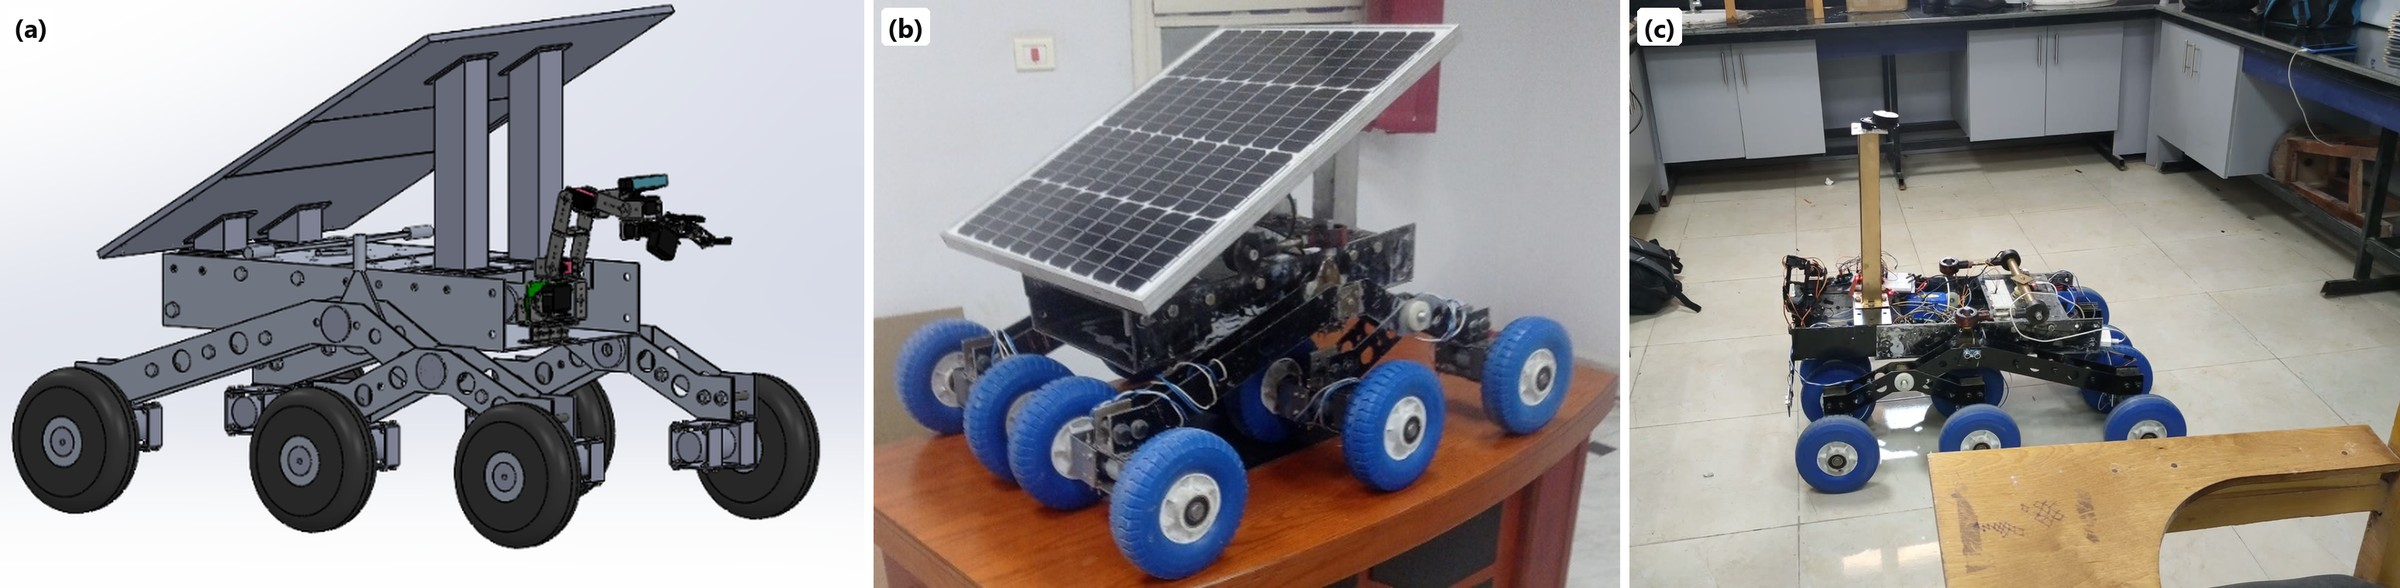
\includegraphics[width=\textwidth]{fig_rover.jpg}
\caption{MISSION~X. (a) SolidWorks model with solar array and 6-DOF arm; (b) as-built rover with the \SI{50}{\watt} panel and doubled \SI{200}{\milli\metre} wheels; (c) navigation configuration with the LDS-01 LiDAR on a mast during the 2023 laboratory trials.}
\label{fig:rover}
\end{figure*}

% =====================================================================
\section{Related Work}
\emph{Rocker--bogie mobility.} The passive rocker--bogie linkage keeps all six wheels in contact with uneven ground without springs, equalising wheel loads and allowing obstacles of the order of a wheel diameter to be climbed~\cite{bickler1989,lindemann2005}. Its kinematics and quasi-static traction have been analysed in detail~\cite{hacot1998,tarokh2005,iagnemma2004}, and comparative mobility metrics for all-terrain chassis are given in~\cite{thueer2010}. Rovers without steering actuators, such as ours, behave as skid-steer vehicles, whose turning is governed by wheel slip; an effective track width calibrated on the actual ground is the standard remedy~\cite{martinez2005,mandow2007}.

\emph{Mapping and navigation.} Two-dimensional LiDAR SLAM is typically solved either by scan-to-map matching, as in Hector SLAM~\cite{kohlbrecher2011}, or with Rao-Blackwellised particle filters~\cite{grisetti2007}; graph-based SLAM Toolbox~\cite{macenski2021} is the reference in ROS~2. Localisation on a known map is commonly done with adaptive Monte-Carlo localisation~\cite{fox2003,thrun2005} and local obstacle avoidance with the dynamic window approach (DWA)~\cite{fox1997}. ROS~\cite{quigley2009} and its successor ROS~2~\cite{macenski2022} with Nav2~\cite{macenski2020} provide these building blocks; physics simulators such as Gazebo~\cite{koenig2004} are the usual test bed.

\emph{Serial links in small spacecraft.} Small spacecraft and their ground segments frequently use byte-oriented framing with flag delimiters and a cyclic redundancy check~\cite{peterson1961,koopman2004}; SLIP/KISS escaping~\cite{rfc1055} and the CCSDS Space Packet~\cite{ccsds133} are common references. The SSP used here was adopted from EgSA's university training programme and frames packets with \texttt{0xC0} flags and a CRC-16.

% =====================================================================
\section{System Overview}
\label{sec:system}
\subsection{Mission and requirements}
The mission concept is autonomous exploration of an unknown environment: build a map with SLAM, navigate it without human input, measure environmental conditions, collect soil samples with a robotic arm, and relay data to a ground station. The derived requirements were: total mass below \SI{40}{\kilo\gram}; stable traverse of slopes and obstacles of the order of the wheel radius; a warm electronics box (WEB) that protects and thermally isolates the avionics; a LiDAR mounted above all structure; ultrasonic sensors around the body for close obstacles; motor cables free of the suspension motion; and solar charging from a panel on top of the rover.

\subsection{Architecture}
Figure~\ref{fig:arch} shows the architecture. A Raspberry~Pi~4 (the ``Brain'') runs Ubuntu and ROS and hosts SLAM, localisation, navigation and the ground-station gateway. Three Arduino microcontrollers handle hard real-time I/O: an Arduino Mega~2560 drives the six motors through three Cytron MDD20A dual drivers and reads the six wheel encoders and ultrasonic sensors (mobility); an Arduino Uno reads the environmental and inertial sensors (payload); a second Uno drives the six arm servos through a PCA9685 PWM controller. The ground link uses an HC-12 \SI{433}{\mega\hertz} transceiver at \SI{9600}{baud}; two ground stations were developed, a LabVIEW application for a PC and a Flutter mobile application that exchanges data with the rover through a Firebase real-time database. Table~\ref{tab:specs} lists the main characteristics and Table~\ref{tab:mass} the mass budget.

\begin{figure*}[t]
\centering
\resizebox{\textwidth}{!}{%
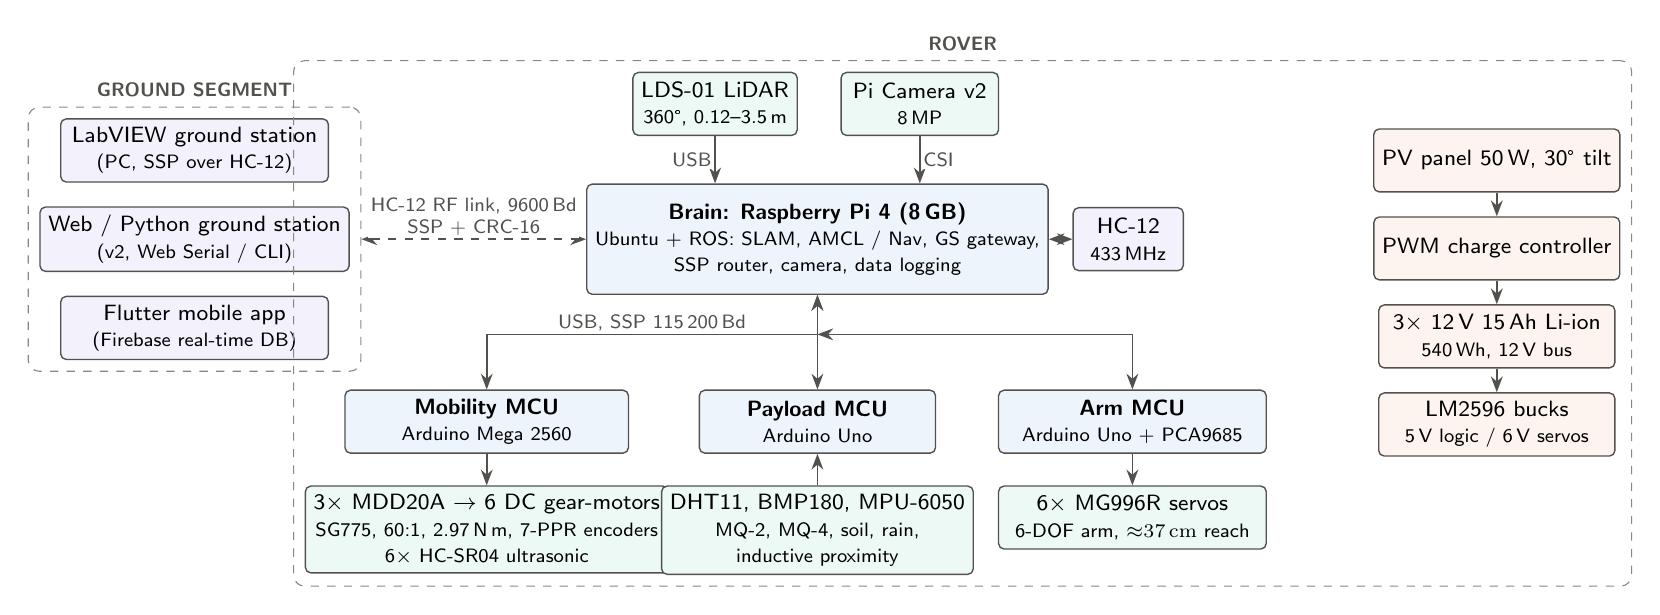
\begin{tikzpicture}[
  font=\sffamily\footnotesize,
  blk/.style={draw=cink2, rounded corners=2pt, fill=white, align=center, minimum height=8mm, inner sep=3pt, line width=0.5pt},
  mcu/.style={blk, fill=cblue!8},
  sens/.style={blk, fill=caqua!8},
  pwr/.style={blk, fill=corange!8},
  gs/.style={blk, fill=cviolet!8},
  lnk/.style={-{Stealth[length=2mm]}, draw=cink2, line width=0.6pt},
  blnk/.style={{Stealth[length=2mm]}-{Stealth[length=2mm]}, draw=cink2, line width=0.6pt},
  lab/.style={font=\sffamily\scriptsize, text=cink2, fill=white, inner sep=1pt}]
% ground segment
\node[gs, minimum width=34mm] (lv) {LabVIEW ground station\\\scriptsize(PC, SSP over HC-12)};
\node[gs, minimum width=34mm, below=3mm of lv] (web) {Web / Python ground station\\\scriptsize(v2, Web Serial / CLI)};
\node[gs, minimum width=34mm, below=3mm of web] (app) {Flutter mobile app\\\scriptsize(Firebase real-time DB)};
\node[draw=cmuted, dashed, rounded corners=4pt, fit=(lv)(web)(app), inner sep=4pt, label={[font=\sffamily\scriptsize\bfseries, text=cink2]above:GROUND SEGMENT}] (gsbox) {};
% brain
\node[mcu, minimum width=46mm, minimum height=14mm, right=30mm of web] (brain) {\textbf{Brain: Raspberry Pi 4 (8\,GB)}\\\scriptsize Ubuntu + ROS: SLAM, AMCL / Nav, GS gateway,\\\scriptsize SSP router, camera, data logging};
\node[sens, above=6mm of brain, xshift=-13mm, minimum width=20mm] (lidar) {LDS-01 LiDAR\\\scriptsize360°, 0.12--3.5\,m};
\node[sens, above=6mm of brain, xshift=13mm, minimum width=20mm] (cam) {Pi Camera v2\\\scriptsize8\,MP};
\node[blk, right=3mm of brain, minimum width=14mm, fill=cviolet!8] (hc) {HC-12\\\scriptsize433\,MHz};
% MCUs
\node[mcu, below=12mm of brain, xshift=-42mm, minimum width=36mm] (mega) {\textbf{Mobility MCU}\\\scriptsize Arduino Mega 2560};
\node[mcu, below=12mm of brain, xshift=0mm, minimum width=30mm] (uno1) {\textbf{Payload MCU}\\\scriptsize Arduino Uno};
\node[mcu, below=12mm of brain, xshift=40mm, minimum width=34mm] (uno2) {\textbf{Arm MCU}\\\scriptsize Arduino Uno + PCA9685};
\node[sens, below=4mm of mega, minimum width=36mm] (drv) {3$\times$ MDD20A $\rightarrow$ 6 DC gear-motors\\\scriptsize SG775, 60:1, 2.97\,N\,m, 7-PPR encoders\\\scriptsize 6$\times$ HC-SR04 ultrasonic};
\node[sens, below=4mm of uno1, minimum width=34mm] (pl) {DHT11, BMP180, MPU-6050\\\scriptsize MQ-2, MQ-4, soil, rain,\\\scriptsize inductive proximity};
\node[sens, below=4mm of uno2, minimum width=34mm] (arm) {6$\times$ MG996R servos\\\scriptsize 6-DOF arm, \SI{\approx 37}{\centi\metre} reach};
% power
\node[pwr, right=24mm of hc, minimum width=30mm, yshift=10mm] (pv) {PV panel 50\,W, 30° tilt};
\node[pwr, below=3mm of pv, minimum width=30mm] (cc) {PWM charge controller};
\node[pwr, below=3mm of cc, minimum width=30mm] (bat) {3$\times$ 12\,V 15\,Ah Li-ion\\\scriptsize 540\,Wh, 12\,V bus};
\node[pwr, below=3mm of bat, minimum width=30mm] (buck) {LM2596 bucks\\\scriptsize 5\,V logic / 6\,V servos};
\node[draw=cmuted, dashed, rounded corners=4pt, fit=(lidar)(cam)(brain)(hc)(drv)(pl)(arm)(pv)(buck), inner sep=4pt, label={[font=\sffamily\scriptsize\bfseries, text=cink2]above:ROVER}] (rv) {};
% links
\draw[lnk] (lidar) -- node[lab, left]{USB} (lidar |- brain.north);
\draw[lnk] (cam) -- node[lab, right]{CSI} (cam |- brain.north);
\draw[blnk] (brain.east) -- (hc.west);
\draw[blnk] (brain.south) -- ++(0,-5mm) -| node[lab, pos=0.25, above]{USB, SSP 115\,200\,Bd} (mega.north);
\draw[blnk] (brain.south) -- (uno1.north);
\draw[blnk] (brain.south) ++(0,-5mm) -| (uno2.north);
\draw[lnk] (mega) -- (drv);
\draw[lnk] (pl) -- (uno1);
\draw[lnk] (uno2) -- (arm);
\draw[lnk] (pv) -- (cc);
\draw[lnk] (cc) -- (bat);
\draw[lnk] (bat) -- (buck);
\draw[blnk, dashed] (gsbox.east) -- node[lab, above, align=center]{HC-12 RF link, 9600\,Bd\\SSP + CRC-16} (brain.west);
\end{tikzpicture}}
\caption{System architecture of MISSION~X. Solid arrows: data links; the HC-12 can alternatively be wired to the mobility MCU, which then answers basic commands on its own (``safe mode'').}
\label{fig:arch}
\end{figure*}

\begin{table}[t]
\centering
\caption{Main characteristics of the as-built rover}
\label{tab:specs}
\footnotesize
\begin{tabular}{@{}p{1.85cm}p{6.45cm}@{}}
\toprule
Dimensions (L$\times$W$\times$H) & $1.02\times0.73\times0.79$\,m \\
Mass & \SI{36.5}{\kilo\gram} \\
Suspension & rocker--bogie, AL-7075 differential pivot \\
Structure & AL-1050 \SI{3}{\milli\metre} sheet, laser-cut; acrylic-lined WEB \\
Wheels & 6 driven + 6 passive twin, \SI{200}{\milli\metre} solid rubber \\
Drive & 6$\times$ SG775 12\,V gear-motor, 60:1, \SI{2.97}{\newton\metre} at 63\,rpm \\
Speed & \SI{0.66}{\metre\per\second} at rated load (\SI{0.87}{\metre\per\second} no load) \\
Odometry & 7-PPR Hall encoders, \SI{0.75}{\milli\metre} per count \\
Computer & Raspberry Pi 4 (8\,GB), ROS; 3 Arduino MCUs \\
Perception & LDS-01 LiDAR, Pi Camera v2, 6$\times$ HC-SR04, MPU-6050 \\
Payload & DHT11, BMP180, MQ-2, MQ-4, soil, rain, metal detector \\
Arm & 6-DOF, 6$\times$ MG996R, PCA9685 \\
Power & \SI{50}{\watt} PV, 3$\times$12\,V 15\,Ah Li-ion (\SI{540}{\watt\hour}) \\
Ground link & HC-12, \SI{433.4}{\mega\hertz}, \SI{20}{dBm}, 9600\,Bd, SSP \\
\bottomrule
\end{tabular}
\end{table}

\begin{table}[t]
\centering
\caption{Mass budget (as built)}
\label{tab:mass}
\footnotesize
\begin{tabular}{@{}lrrr@{}}
\toprule
Item & Unit [kg] & Qty & Total [kg] \\
\midrule
Structure (WEB, rocker--bogie) & -- & -- & 11.0 \\
Drive motors & 1.0 & 6 & 6.0 \\
Wheels (driven + twin) & 0.5 & 12 & 6.0 \\
Solar array with support & 4.0 & 1 & 4.0 \\
Batteries & 1.0 & 3 & 3.0 \\
Electronics and harness & -- & -- & 3.0 \\
Differential pivot & -- & -- & 2.0 \\
Robotic arm & 1.5 & 1 & 1.5 \\
\midrule
Total & & & 36.5 \\
\bottomrule
\end{tabular}
\end{table}

% =====================================================================
\section{Mechanical Design and Mobility}
\label{sec:mech}
\subsection{Rocker--bogie chassis}
Each side of the rover has a rocker, carrying the front wheel and pivoting on the body, and a bogie, carrying the middle and rear wheels and pivoting on the rocker. A differential bar on top of the WEB links the two rockers so that the body pitch is the average of the two rocker angles; it was made of AL-7075, while the WEB and the rocker--bogie links were laser-cut from \SI{3}{\milli\metre} AL-1050 sheet and welded. Each rocker--bogie joint uses two 6203 bearings. The motor housings (``motor boxes'') clamp the SG775 gear-motors, and the WEB is lined with \SI{1}{\milli\metre} acrylic for thermal isolation.

Integration revealed four structural problems, which shaped the final design: (i) the first differential pivot was too weak and was re-made thicker in AL-7075; (ii) the rocker--bogie legs bent and vibrated under load and had to be stiffened with ten additional bolts; (iii) a small-diameter spherical joint for the pivot was not available and a larger one had to be used; (iv) the first \SI{120}{\milli\metre} wheels were too small, and with the heavier final configuration the cantilevered motor boxes tilted. The fix was \SI{200}{\milli\metre} wheels doubled at every station: one driven and one passive twin wheel on each side of every motor box.

\subsection{Mobility analysis}
The original design sized the motors by requiring each wheel to lift one sixth of the weight vertically, $T = (mg/6)\,r_w = \SI{5.97}{\newton\metre}$, i.e.\ twice the rated torque of the selected motor. This criterion corresponds to the limiting case of a wheel climbing a vertical riser; it does not describe slopes or steps. We therefore re-assessed mobility with two quasi-static models. With the load shared by six driven wheels, the torque per wheel needed to climb a slope $\theta$ at constant speed is
\begin{equation}
T(\theta) = \tfrac{1}{6}\,m g\,(\sin\theta + C_{rr}\cos\theta)\,r_w,
\label{eq:grade}
\end{equation}
with rolling-resistance coefficient $C_{rr}=0.05$~\cite{wong2008}. On flat ground this is only \SI{0.30}{\newton\metre} (\SI{10}{\percent} of rated torque). Fig.~\ref{fig:mobility}(a) shows that the rated torque suffices up to \SI{26.9}{\degree} on Earth. With wheel--ground friction $\mu$ the traction limit is $\tan\theta=\mu-C_{rr}$, i.e.\ \SI{36.9}{\degree}, \SI{28.8}{\degree} and \SI{19.3}{\degree} for $\mu = 0.8$, 0.6 and 0.4. Under Mars or Moon gravity torque never limits, and the rover is traction-limited at every slope.

For step climbing, the front wheel touches the step edge at angle $\alpha$ from the vertical, $\cos\alpha = (r_w-h)/r_w$ for $h<r_w$. With wheel load $W_f$ and the horizontal push $P$ exerted on each front wheel by the four rear wheels, equilibrium gives the edge normal and tangential forces
\begin{equation}
N = P\sin\alpha + W_f\cos\alpha,\qquad F = W_f\sin\alpha - P\cos\alpha,
\label{eq:step}
\end{equation}
which must satisfy $F\le\mu N$ and $F r_w\le T$, with $P = 2\min(\mu W/6,\,T/r_w) - 2C_{rr}W/6$. Fig.~\ref{fig:mobility}(b) gives the largest climbable step: at the rated torque the rover is torque-limited to \SI{55}{\milli\metre} ($\approx 0.55\,r_w$) for $\mu\ge0.5$. Climbing a step of one wheel radius, the ``half a wheel'' claimed in the original report, needs short bursts near stall torque and $\mu\ge0.74$; six stalled motors then draw about \SI{84}{\ampere} from the battery bus. When torque does not bind, as on Earth at stall or on Mars at rated torque, all forces scale with the weight and the limit depends on $\mu$ alone. These quasi-static results bound, but do not replace, field tests on representative terrain.

\begin{figure}[t]
\centering
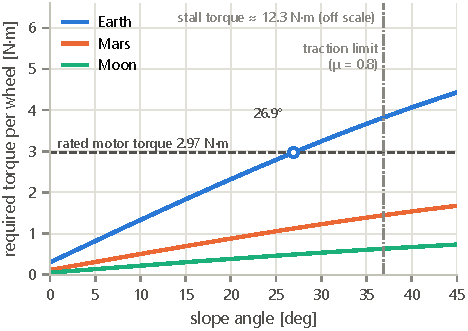
\includegraphics[width=\columnwidth]{fig_gradeability.pdf}\\[-1mm]
{\footnotesize (a)}\\[1mm]
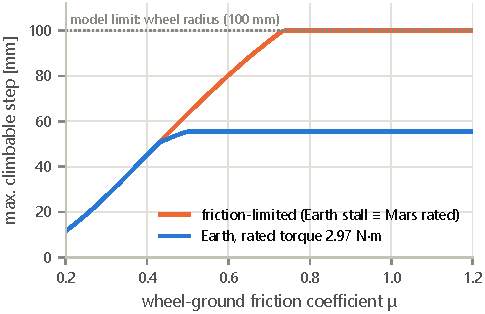
\includegraphics[width=\columnwidth]{fig_step_climb.pdf}\\[-1mm]
{\footnotesize (b)}
\caption{Mobility analysis. (a) Torque per wheel required by Eq.~\eqref{eq:grade} versus slope under Earth, Mars and Moon gravity. (b) Largest step that both front wheels can climb according to Eq.~\eqref{eq:step}, versus friction coefficient.}
\label{fig:mobility}
\end{figure}

\subsection{Structural analysis re-assessed}
The team analysed a front-impact load case of the complete assembly in SolidWorks (Fig.~\ref{fig:fea}). The report concluded that the maximum stress is below the yield strength. Reading the result legend shows otherwise: the peak nodal von~Mises stress is \SI{44.1}{\mega\pascal}, while the yield strength of the library material AL-1050 (annealed) is \SI{27.6}{\mega\pascal}, a minimum factor of safety of 0.62. The peaks are local, at joints and fixtures; most of the structure stays below \SI{13}{\mega\pascal}, and the maximum displacement is only \SI{0.13}{\milli\metre}. The prediction nevertheless agrees with the bending of the rocker--bogie legs observed during integration. A strain-hardened temper of AL-1050 (H14/H24) or a 5xxx/6xxx alloy for the legs, or local doubler plates at the joints, would restore a factor of safety above two. We report this explicitly because a misread FEA legend is an easy and consequential mistake.

\begin{figure}[t]
\centering
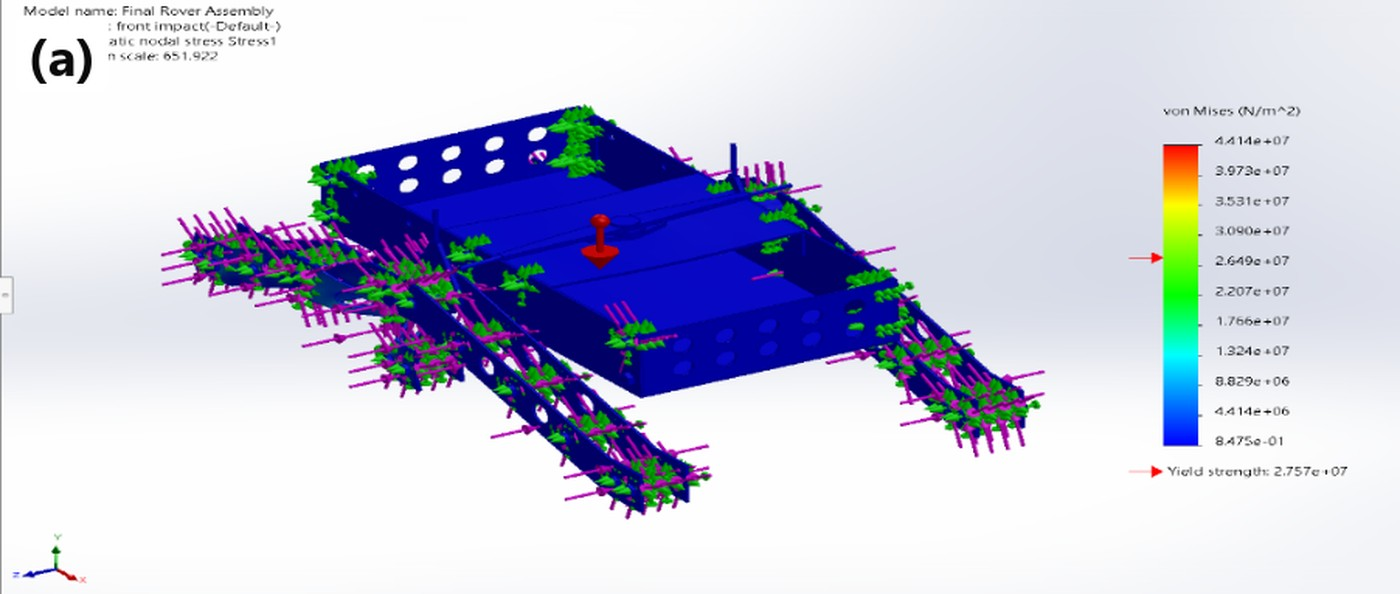
\includegraphics[width=\columnwidth]{fig_fea.jpg}
\caption{Team's SolidWorks static study (front impact): von~Mises stress with legend maximum \SI{44.1}{\mega\pascal} and library yield strength \SI{27.6}{\mega\pascal} (red arrow).}
\label{fig:fea}
\end{figure}

% =====================================================================
\section{Electrical Power}
\label{sec:power}
The \SI{50}{\watt} panel, tilted \SI{30}{\degree}, charges three \SI{12}{\volt} \SI{15}{\ampere\hour} Li-ion packs through a \SI{10}{\ampere} PWM charge controller. LM2596 buck converters supply the \SI{5}{\volt} logic and \SI{6}{\volt} servo rails, and the motor drivers run directly from the \SI{12}{\volt} bus. The original budget (\SI{365}{\watt}, ``\SI{35.3}{\ampere}'') added currents drawn from different voltage rails, used \SI{0.2}{\ampere} per Hall encoder instead of the \SI{14}{}--\SI{20}{\milli\ampere} of the datasheet, included sensors that were never fitted (a Kinect and a YDLIDAR~G4), and assumed all six motors at rated load continuously. It also predicted a 12-hour solar recharge, which corresponds to the panel delivering its rated power continuously.

We rebuilt the budget per rail, referred it to the battery bus with \SI{85}{\percent} converter efficiency, and evaluated it for five operating modes (Fig.~\ref{fig:power}). Motor current is modelled as linear in torque between the no-load and rated points. On flat ground the six motors draw \SI{61}{\watt} together, dominated by the no-load current of the gearboxes. With \SI{432}{\watt\hour} usable capacity (\SI{80}{\percent} depth of discharge) the rover runs \SI{5.5}{\hour} in continuous flat traverse, \SI{2.1}{\hour} in rough terrain or skid-steer turns at \SI{60}{\percent} of rated torque, and \SI{6.7}{\hour} on a representative sortie (\SI{40}{\percent} traverse, \SI{10}{\percent} rough terrain, \SI{50}{\percent} science stops; \SI{65}{\watt} average). At Beni-Suef (\SI{\approx 6}{} peak-sun hours) the panel yields about \SI{186}{\watt\hour} per day through the PWM controller and about \SI{240}{\watt\hour} with an MPPT controller. A full recharge therefore takes about two sunny days, not 12~hours. On Mars, where daily insolation at low latitudes is of the order of \SI{3}{\kilo\watt\hour\per\square\metre} for moderate dust opacity~\cite{appelbaum1990} (about three equivalent peak-sun hours), the recharge would grow to roughly 4--5 sols.

\begin{figure*}[t]
\centering
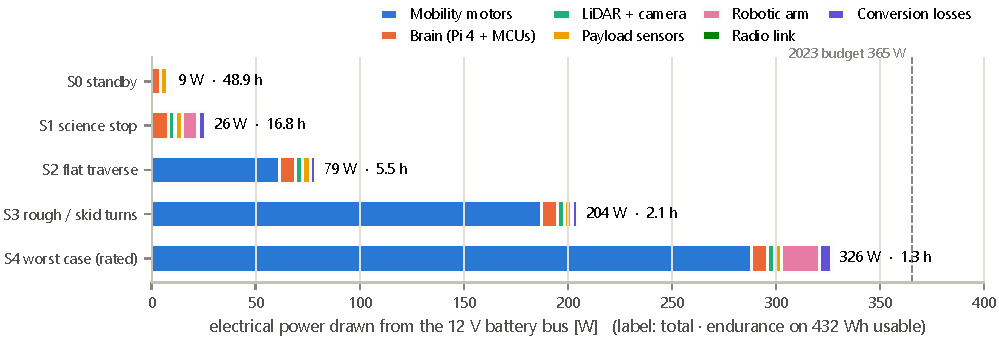
\includegraphics[width=\textwidth]{fig_power_modes.pdf}
\caption{Corrected power budget by operating mode, referred to the \SI{12}{\volt} battery bus, with endurance on \SI{432}{\watt\hour} usable energy. The dashed line marks the original 2023 budget.}
\label{fig:power}
\end{figure*}

% =====================================================================
\section{Avionics and Software}
\label{sec:avionics}
\subsection{As-built software (2023)}
The Brain ran ROS Noetic on Ubuntu~20.04. The LDS-01 LiDAR~\cite{lds01} fed Hector SLAM~\cite{kohlbrecher2011}, which builds an occupancy grid from LiDAR scan matching alone and so suited a rover whose encoder data were not yet integrated. Saved maps were then used with \texttt{map\_server}, AMCL~\cite{fox2003} and \texttt{move\_base} with the DWA local planner~\cite{fox1997}, targets being set in RViz. The payload MCU published its readings on ROS topics through \texttt{rosserial}, and the Brain bridged ground-station commands to the subsystems. The mobility MCU additionally implemented a reactive ultrasonic obstacle-avoidance behaviour, used when the rover was commanded to ``start scan'' without the Brain. The 6-DOF arm was driven from a table of calibrated servo angles, and the payload firmware used one C++ class per sensor.

\subsection{Ground segment}
The LabVIEW ground station builds SSP command frames, computes the CRC, and decodes the responses into gauges, charts and an image view. Supported commands are \emph{ping}, \emph{get telemetry}, \emph{capture image}, \emph{get image} (a $100\times100$ grey image in 50 packets of \SI{200}{\byte}), \emph{start scan}, \emph{stop scan} and \emph{collect object}. The Flutter application exposes the same commands and plots the sensor histories by writing and listening to ``commands'' and ``sensors'' nodes of a Firebase real-time database. This allows control over the Internet whenever the rover has connectivity.

\subsection{Simple Serial Protocol}
An SSP frame (Fig.~\ref{fig:ssp}) is delimited by \texttt{0xC0} flags and carries destination and source addresses, a packet type, a length byte, up to \SI{255}{\byte} of data and a CRC-16. The CRC uses the generator $x^{16}+x^{12}+x^5+1$ with zero initial value (CRC-16/XMODEM), which detects all errors of up to three bits and all bursts of up to 16 bits in frames of this length~\cite{peterson1961,koopman2004}. The audit in Section~\ref{sec:comm} led to a revised ICD (v2.0) that fixes the ambiguous points of the original implementation. These include the CRC byte order (low byte first, as transmitted by the LabVIEW station), address handling in replies, a normative length-driven receiver with resynchronisation and a per-type length plausibility check, optional SLIP-style transparency~\cite{rfc1055}, and new packet types for velocity commands with a watchdog, wheel odometry, ranges, IMU and environment telemetry, arm control and emergency stop. The legacy commands and frame format are unchanged, so the LabVIEW station keeps working.

\begin{figure}[t]
\centering
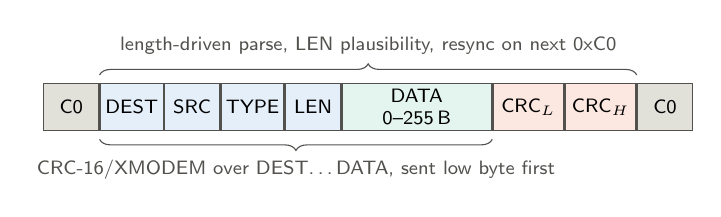
\begin{tikzpicture}[font=\sffamily\scriptsize, x=1mm, y=1mm,
  f/.style={draw=cink2, line width=0.5pt, minimum height=6mm, inner sep=0pt, align=center, anchor=west}]
\def\h{6}
\node[f, minimum width=7mm, fill=cgrid] (a) at (0,0) {C0};
\node[f, minimum width=8mm, fill=cblue!12] (b) at (a.east) {DEST};
\node[f, minimum width=7mm, fill=cblue!12] (c) at (b.east) {SRC};
\node[f, minimum width=8mm, fill=cblue!12] (d) at (c.east) {TYPE};
\node[f, minimum width=7mm, fill=cblue!12] (e) at (d.east) {LEN};
\node[f, minimum width=19mm, fill=caqua!12] (g) at (e.east) {DATA\\0--255\,B};
\node[f, minimum width=9mm, fill=corange!15] (h) at (g.east) {CRC$_L$};
\node[f, minimum width=9mm, fill=corange!15] (i) at (h.east) {CRC$_H$};
\node[f, minimum width=7mm, fill=cgrid] (j) at (i.east) {C0};
\draw[decorate, decoration={brace, amplitude=4pt, mirror}, cink2] ([yshift=-1mm]b.south west) -- node[below=4pt, align=center]{CRC-16/XMODEM over DEST\dots DATA, sent low byte first} ([yshift=-1mm]g.south east);
\draw[decorate, decoration={brace, amplitude=4pt}, cink2] ([yshift=1mm]b.north west) -- node[above=4pt, align=center]{length-driven parse, LEN plausibility, resync on next 0xC0} ([yshift=1mm]i.north east);
\end{tikzpicture}
\caption{SSP frame (ICD v2.0, wire-compatible with the 2023 ground station). Example: \texttt{C0 01 0B 0F 00 7B 96 C0} is a \emph{get telemetry} request from the ground station (0x0B) to the rover (0x01).}
\label{fig:ssp}
\end{figure}

\subsection{ROS 2 reference stack}
ROS Noetic reached end of life in 2025 and the original ROS code was not archived with the project. We therefore re-implemented the pipeline on ROS~2 Jazzy~\cite{macenski2022} (Table~\ref{tab:ros}). \texttt{rosserial} has no maintained ROS~2 counterpart for 8-bit AVR boards, and micro-ROS targets 32-bit microcontrollers. Instead, every MCU now speaks SSP over USB and three bridge nodes translate frames to standard messages, so a single protocol and a single tested library serve both the ground link and the on-board buses. A \texttt{robot\_localization} EKF fuses wheel odometry with the gyro, SLAM Toolbox~\cite{macenski2021} replaces Hector SLAM, and Nav2~\cite{macenski2020} with the DWB controller replaces \texttt{move\_base}. Its costmaps add a range-sensor layer for the six ultrasonic sensors, motivated by Section~\ref{sec:results}. A frontier-based explorer implements ``start scan'', and a gateway node implements the ground-station command set. The same bridges are driven by a lightweight simulator (Section~\ref{sec:results}), so SLAM, navigation and the gateway run unchanged in simulation.

\begin{table}[t]
\centering
\caption{2023 software pipeline and its ROS 2 re-implementation}
\label{tab:ros}
\footnotesize
\begin{tabular}{@{}lll@{}}
\toprule
Function & 2023 (ROS Noetic) & v2 (ROS 2 Jazzy) \\
\midrule
MCU bridge & rosserial & SSP bridges (USB) \\
Odometry & -- (LiDAR only) & wheel + gyro EKF \\
SLAM & Hector SLAM & SLAM Toolbox \\
Localisation & AMCL & Nav2 AMCL \\
Local planner & move\_base / DWA & Nav2 / DWB \\
Costmap sensors & LiDAR & LiDAR + 6 ultrasonic \\
Exploration & reactive (MCU) & frontier explorer \\
GS gateway & ad hoc & SSP gateway node \\
\bottomrule
\end{tabular}
\end{table}

% =====================================================================
\section{Communication Link and Interface Audit}
\label{sec:comm}
\subsection{Link budget}
The HC-12 transmits \SI{20}{dBm} at \SI{433.4}{\mega\hertz}. In its default FU3 mode a \SI{9600}{baud} serial rate maps to a \SI{15}{\kilo\bit\per\second} air rate, for which the receiver sensitivity is \SI{-112}{dBm}~\cite{hc12}. With the antennas only \SI{0.8}{\metre} (rover) and \SI{1.0}{\metre} (ground) above the ground, the two-ray model~\cite{rappaport2002} applies beyond \SI{14.5}{\metre} and path loss grows with \SI{40}{\decibel} per decade. Assuming \SI{0}{dBi} spring antennas, \SI{2}{\decibel} system losses and a \SI{10}{\decibel} fade margin, the range is \SI{\approx 0.9}{\kilo\metre} (Fig.~\ref{fig:link}), in line with the vendor's \SI{1}{\kilo\metre} figure. Dropping to the \SI{5}{\kilo\bit\per\second} air rate extends it to \SI{1.2}{\kilo\metre}; \SI{236}{\kilo\bit\per\second} reduces it to \SI{0.45}{\kilo\metre}. At \SI{9600}{baud} a ping takes \SI{8.3}{\milli\second} to serialise and a v2 telemetry reply \SI{67}{\milli\second}. A legacy $100\times100$ image needs \SI{10.8}{\second}, a reminder that imaging over such a link must be compressed or scheduled.

\begin{figure}[t]
\centering
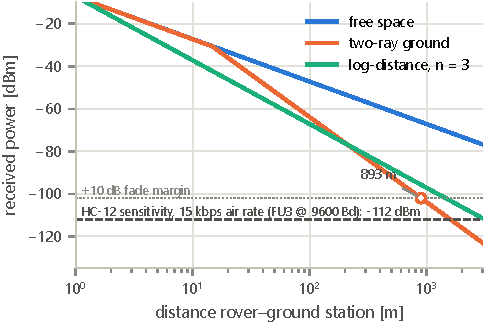
\includegraphics[width=\columnwidth]{fig_link_budget.pdf}
\caption{HC-12 received power versus distance for three path-loss models. The marker shows the two-ray range with a \SI{10}{\decibel} fade margin at the \SI{15}{\kilo\bit\per\second} air rate.}
\label{fig:link}
\end{figure}

\subsection{Interface defects}
We inspected the three SSP implementations (LabVIEW on the ground, Python on the Brain and C++ on the Arduino) and checked them against frames captured during the 2023 tests. This uncovered the defects listed in Table~\ref{tab:defects}. The most instructive is D1. The LabVIEW station and the Python code send the CRC low byte first, which we verified against a captured LabVIEW frame (\texttt{CRC = 0x967B} sent as \texttt{7B 96}), whereas the Arduino code appended it high byte first. The mismatch went unnoticed because the Arduino discarded the result of its own CRC check (D2) and dispatched on whatever eight bytes it had read. To make telemetry ``work'', a constant reply frame had been hard-coded (D6). Each defect alone is mundane; together they produced a link that appeared to work in the laboratory while silently accepting corrupted commands. All defects are fixed in the v2 firmware and Brain software, which are checked against one shared set of test vectors: a Python reference implementation and the embedded C++ decoder must yield identical frames and statistics on \num{192} corrupted streams.

\begin{table}[t]
\centering
\caption{Interface defects found in the 2023 implementation}
\label{tab:defects}
\footnotesize
\setlength{\tabcolsep}{3pt}
\begin{tabular}{@{}p{0.6cm}>{\raggedright\arraybackslash}p{3.5cm}>{\raggedright\arraybackslash}p{3.6cm}@{}}
\toprule
\# & Defect & Consequence \\
\midrule
D1 & CRC byte order differs (Arduino vs.\ LabVIEW/Python) & frames rejected across implementations \\
D2 & CRC check result ignored & corrupted commands executed \\
D3 & fixed 8-byte reads, no framing state & one lost byte misaligns frames \\
D4 & reply source/destination not swapped & replies addressed to the rover \\
D5 & \texttt{malloc} per command, never freed & heap exhaustion on 8\,KB SRAM \\
D6 & telemetry reply hard-coded & data not from sensors \\
D8 & 8-bit range, \texttt{pulseIn} without timeout & ranges wrap; loop blocked \SI{1}{\second} \\
D11 & no command watchdog & rover keeps driving on link loss \\
\bottomrule
\end{tabular}
\end{table}

\subsection{Fault-injection study}
To quantify the safety impact of D2--D3 we sent \num{40000} random legacy commands per operating point through a channel with independent bit errors or byte drops. Each stream was fed to an emulation of the 2023 receiver (``read eight bytes when more than five are available, dispatch on the type byte, flush'') and to the v2 receiver. Fig.~\ref{fig:mc} shows the outcome. The 2023 receiver often executes a \emph{different} command from the one sent: \SI{0.09}{\percent} of commands at a bit error rate of $10^{-3}$, and \SI{3.1}{\percent} and \SI{8.9}{\percent} at byte-drop probabilities of 1 and \SI{3}{\percent}. A dropped byte shifts the length field into the type position, and a single bit flip can turn \emph{capture image} (\texttt{0x0C}) into \emph{stop scan} (\texttt{0x1C}). The v2 receiver rejects every corrupted frame, so the ground station can retry, and executed no wrong command in \num{520000} trials. The price is that a corrupted frame is now always discarded instead of being executed by chance, which is the intended behaviour for a space link.

\begin{figure*}[t]
\centering
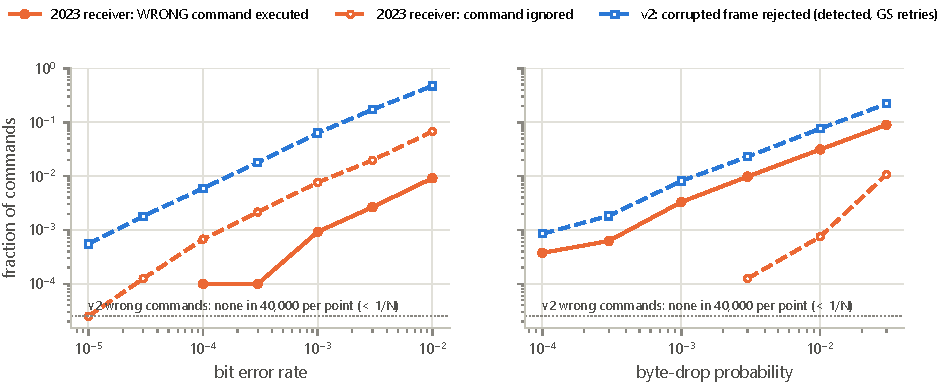
\includegraphics[width=\textwidth]{fig_protocol_mc.pdf}
\caption{Monte-Carlo fault injection (\num{40000} commands per point) for the 2023 receiver and the v2 receiver, under random bit errors (left) and byte drops (right). The v2 receiver executed no wrong command at any point.}
\label{fig:mc}
\end{figure*}

% =====================================================================
\section{Experimental and Simulation Results}
\label{sec:results}
\subsection{Laboratory demonstration (2023)}
The integrated rover was demonstrated in the faculty laboratory (Fig.~\ref{fig:real}). Driven by keyboard tele-operation, it mapped the laboratory with Hector SLAM; the map captures the walls, the benches and most furniture (Fig.~\ref{fig:real}a). With the saved map, AMCL and \texttt{move\_base}, the rover then navigated autonomously to goals set in RViz between benches and chairs (Fig.~\ref{fig:real}c,d). In the same tests the payload readings were published on ROS topics, and the LabVIEW ground station exchanged \emph{ping} and \emph{telemetry} frames with the rover over the HC-12 link. These trials were qualitative demonstrations: no ground-truth trajectory or repeated trials were recorded, which motivated the simulation study below. The team also reported two limitations that the study addresses: small, low obstacles cannot be seen by the LiDAR on top of the rover, and the delay between an ultrasonic detection and the motor command of the MCU-based avoidance degraded the motion.

\begin{figure*}[t]
\centering
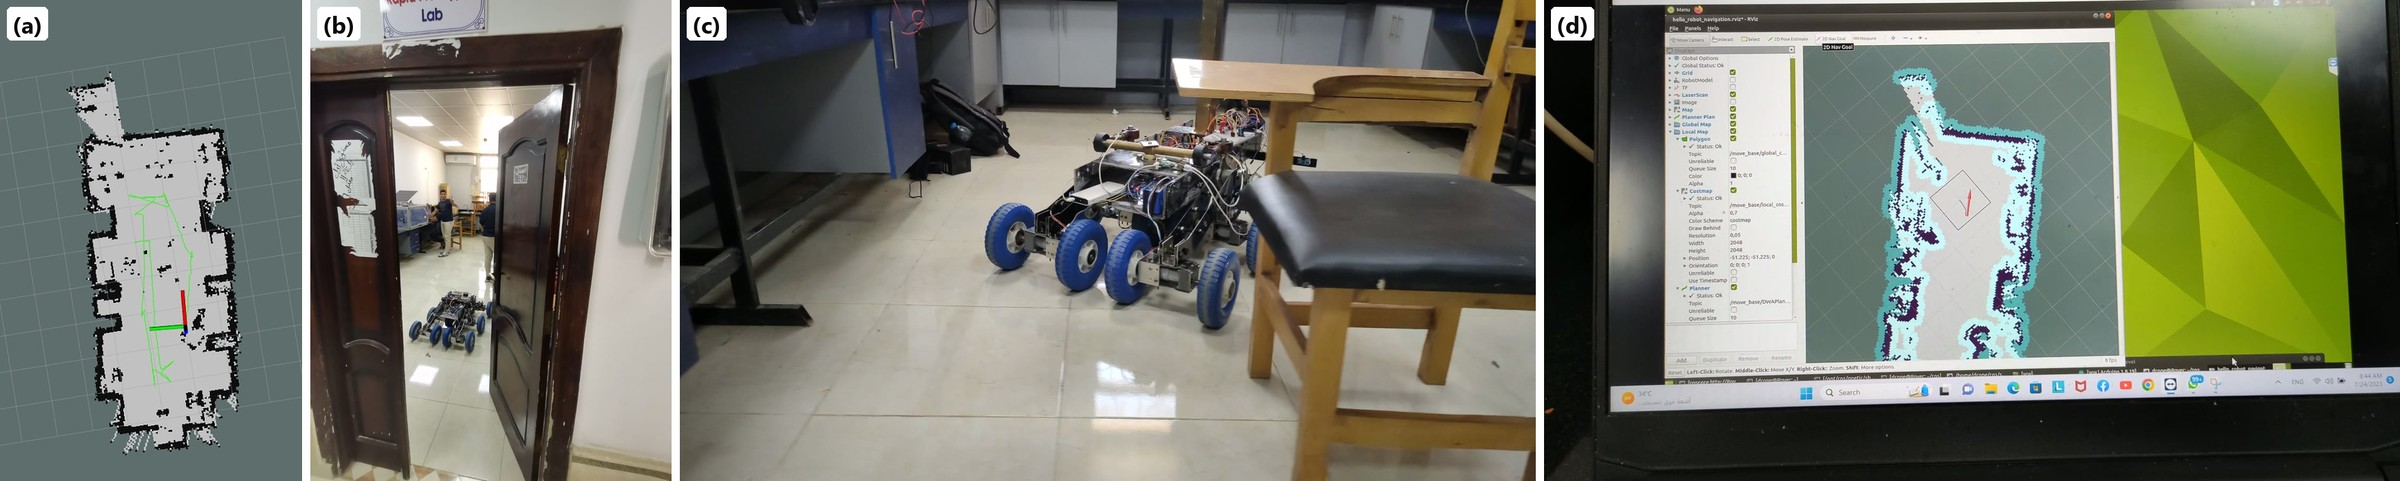
\includegraphics[width=\textwidth]{fig_real_results.jpg}
\caption{2023 laboratory trials. (a) Hector SLAM map of the laboratory with the trajectory (green); (b) the rover entering the laboratory during mapping; (c) autonomous navigation between benches and chairs; (d) RViz with the saved map, AMCL pose and \texttt{move\_base} costmaps during the run.}
\label{fig:real}
\end{figure*}

\subsection{Digital twin}
The simulator is a pure-Python (NumPy) 2.5-D model that runs on any PC and on the rover's computer. The world is a grid holding the height of the obstacle standing in each \SI{2}{\centi\metre} cell. The skid-steer vehicle turns with an effective track $\chi b$ whose true value differs from the controller's nominal one ($\chi_\text{true} = 1.1\,\chi_\text{nom}$ here). Side speeds follow a first-order lag with an acceleration limit and the motors' torque--speed line, and the model includes random longitudinal slip and occasional free-spinning wheels. Encoders are quantised to \num{840} counts per revolution, and the gyro has a constant bias plus white noise. The LDS-01 model casts 360 beams at \SI{1}{\degree} and \SI{5}{\hertz} over \SI{0.12}{}--\SI{3.5}{\metre}, with range noise $\sigma = \SI{10}{\milli\metre}$ below \SI{0.5}{\metre} and \SI{1.75}{\percent} of range above, and \SI{2}{\percent} dropouts. It sees only obstacles that reach its \SI{0.62}{\metre} scan plane. Each HC-SR04 model is a \SI{15}{\degree} cone sampled by five rays at \SI{0.25}{\metre} height; it sees an obstacle only when the obstacle's top is above the lower edge of the cone. The laboratory world, $10\times7$\,m, contains benches, a central island, wooden chairs whose seats lie below the LiDAR plane, and low crates.

\subsection{Mapping}
The rover drove a \SI{31.5}{\metre} loop through the simulated laboratory in \SI{157}{\second} (785 scans). The same sensor stream fed two estimators: mapping at the wheel-odometry pose (uncalibrated $\chi$), and Hector-style multi-resolution Gauss--Newton scan-to-map matching~\cite{kohlbrecher2011} at \SI{5}{\centi\metre} resolution, with the odometry increment as prior,
\begin{equation}
\xi^\ast = \arg\min_{\xi}\sum_i \big[1 - M(S_i(\xi))\big]^2,
\end{equation}
where $M$ is the bilinearly interpolated occupancy map and $S_i(\xi)$ the $i$-th scan endpoint transformed by pose $\xi$. Over eight runs with different noise seeds (mean $\pm$ s.d.; Fig.~\ref{fig:slam} shows one), scan matching reduced the RMS absolute trajectory error from \odoATEsd\,m to \slamATEsd\,m and the heading error from \odoHead\textdegree{} to \slamHead\textdegree. Mapped obstacle cells lay \slamMapAcc\,cm on average from the true obstacles, and \slamCompl\,\% of the observed obstacle cells were recovered within \SI{10}{\centi\metre}; for the odometry-only map these figures are \odoMapAcc\,cm and \odoCompl\,\%. The residual offset of a few centimetres is the known half-cell bias of grid scan matching.

\begin{figure*}[t]
\centering
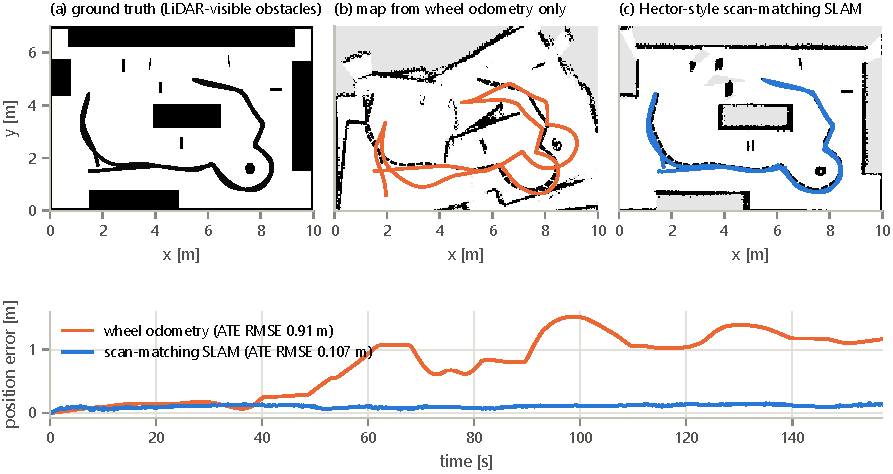
\includegraphics[width=\textwidth]{fig_slam.pdf}
\caption{Simulated mapping run. (a) Obstacles visible in the LiDAR plane and true trajectory; (b) map built at the wheel-odometry pose; (c) map and trajectory from scan-matching SLAM (dashed: ground truth); bottom: position error over time.}
\label{fig:slam}
\end{figure*}

\subsection{Odometry}
Because the rover has no steered wheels, its odometry is skid-steer odometry,
\begin{equation}
v_{L,R} = v \mp \omega\,\chi b/2,\qquad \Delta s_{L,R} = \operatorname{med}\left(\Delta s_{1},\Delta s_{2},\Delta s_{3}\right)_{L,R},
\end{equation}
where the median of the three wheels on each side rejects a single slipping or airborne wheel, which is common on a rocker--bogie. Over 20 runs of a twice-driven \SI{4}{\metre} square (\SI{31}{\metre}), the 2023-style estimate (mean of the three wheels, nominal $\chi$) ended \SI{11.4}{\percent} of the distance travelled away from the truth (Fig.~\ref{fig:odo}). Calibrating $\chi$ with a commanded \SI{360}{\degree} spin reduced the error to \SI{1.4}{\percent}, the median fusion to \SI{1.25}{\percent}, and taking the heading from the bias-compensated gyro to \SI{0.5}{\percent}. Heading, not distance, dominates dead-reckoning error on a skid-steer rover. Hence the EKF in the ROS~2 stack takes its yaw rate from the IMU.

\begin{figure*}[t]
\centering
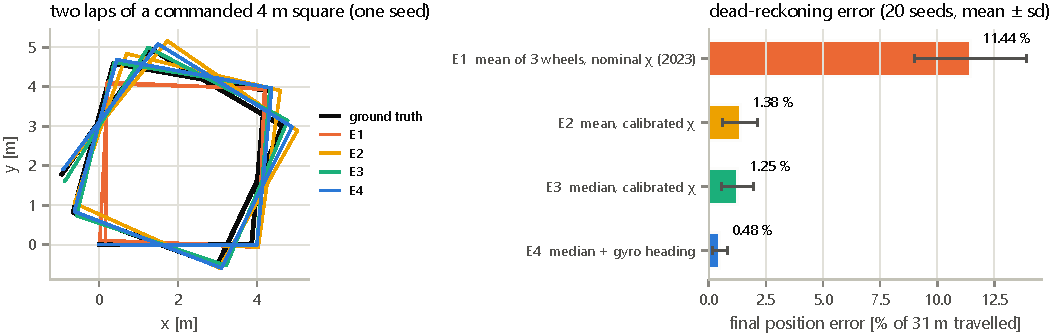
\includegraphics[width=\textwidth]{fig_odometry.pdf}
\caption{Dead reckoning on a twice-driven \SI{4}{\metre} square. Left: trajectories of one run; right: final position error over 20 runs (mean $\pm$ s.d.).}
\label{fig:odo}
\end{figure*}

\subsection{Obstacles below the LiDAR plane}
To isolate the effect of sensor placement, the rover drove straight at \SI{0.35}{\metre\per\second} towards a $0.30\times0.30$\,m obstacle \SI{2.6}{\metre} ahead. We varied the obstacle height from \SI{0.10}{} to \SI{0.70}{\metre} and its lateral offset from \SI{-0.6}{} to \SI{0.6}{\metre}, with three noise seeds per cell (351 runs per configuration). A reactive safety layer equivalent to a collision-monitor stop zone stopped the rover whenever a sensed point lay in its swept corridor less than \SI{0.35}{\metre} ahead of the bumper. With the LiDAR alone, every obstacle below the scan plane that intersected the path was hit: 231 collisions (Fig.~\ref{fig:obst}a). Adding the ultrasonic ring as instantaneous readings stopped the rover for obstacles of \SI{0.25}{\metre} and taller but still left 75 collisions. Obstacles of \SI{0.20}{\metre} and below drop under the lower edge of the \SI{15}{\degree} sonar cone in the last \SI{0.4}{}--\SI{1.1}{\metre} and are forgotten (Fig.~\ref{fig:obst}b). Keeping the sonar detections for \SI{10}{\second} in the odometry frame, as a costmap range layer does, removed every collision: all 297 runs whose obstacle intersected the path ended in a safe stop. The rover stopped on average \SI{0.28}{\metre} short of the obstacle. Because a sonar echo does not tell where in the cone the reflector is, persistence costs 42 conservative stops for obstacles that would have cleared the body (Fig.~\ref{fig:obst}c). This is the configuration adopted in the ROS~2 costmaps.

\begin{figure*}[t]
\centering
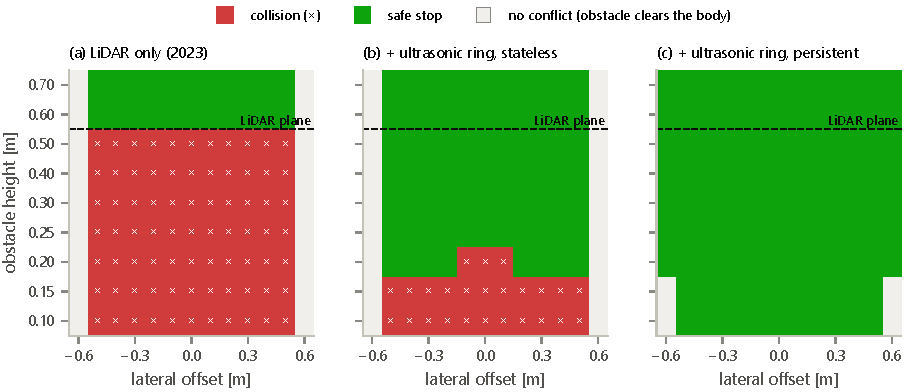
\includegraphics[width=\textwidth]{fig_obstacle_detection.pdf}
\caption{Approach tests against obstacles of varying height and lateral offset (worst outcome of three seeds per cell). (a) LiDAR only; (b) LiDAR and ultrasonic ring, instantaneous readings; (c) LiDAR and ultrasonic ring with persistent detections.}
\label{fig:obst}
\end{figure*}

% =====================================================================
\section{Discussion and Lessons Learned}
\label{sec:discussion}
\emph{Write the ICD first.} Three independent SSP implementations disagreed on one byte order, and the disagreement survived integration because a check was disabled to make things work. A one-page ICD with test vectors, run against every implementation, would have caught it on the first day. It now costs less than a minute per build.

\emph{Read the analysis you run.} Both the motor sizing and the FEA conclusion in the original report were contradicted by their own numbers: the torque criterion modelled a vertical climb, and the stress legend exceeded the library yield strength. In each case the prototype behaved as the corrected analysis predicts: it drove without difficulty on the laboratory floor, where only about \SI{10}{\percent} of rated torque is needed, and its legs bent under load.

\emph{Budgets are per rail and per mode.} Adding currents across rails and assuming continuous worst-case load gave a budget that was too pessimistic in endurance and too optimistic in recharge time. Mode-based budgets referred to the battery bus are no harder to build and give numbers an operator can plan with.

\emph{Mount sensors for the obstacles you have.} A LiDAR on a mast gives clean, unobstructed scans but is blind to anything lower than its scan plane, and on a rover many hazards are low. Sonar fills the gap only if its detections persist; ideally the sensors are tilted downward or complemented by a depth camera.

\emph{Limitations.} The real-world results are qualitative demonstrations on a flat laboratory floor; no tests on loose soil, slopes or steps were made, and the mobility and power figures are analytical. The simulation is a 2.5-D model with sensor models taken from datasheets rather than measured, and the scan matcher is a re-implementation of the Hector front end. The ROS~2 stack has been checked with unit tests, static validation and a simulated node layer, but not yet run on the rover. These are the next steps.

% =====================================================================
\section{Conclusion}
MISSION~X shows that a six-wheel rocker--bogie rover with LiDAR-based autonomy, an environmental payload, a sampling arm, solar power and a two-way ground link can be designed, built and operated by an undergraduate team with low-cost commercial components. Our post-hoc verification turned the project report into reusable engineering data. It quantified gradeability, step climbing, endurance and radio range; it exposed and corrected interface defects that had made the command link silently unsafe; and it used a digital twin to show which changes matter most: scan matching for mapping, a calibrated skid-steer model with gyro heading for odometry, and persistent ultrasonic sensing for low obstacles. Future work will deploy the ROS~2 stack on the rover, add a downward-looking depth camera and vision-based sample detection for autonomous collection, measure traction and power on sand and slopes, and move the ground link to a CCSDS-compatible packet structure~\cite{ccsds133}.

\section*{Data and Code Availability}
The firmware, the ROS~2 stack, the ground-station tools, the scripts that produce every figure and number in this paper, and the original 2023 project files (reports, CAD models, LabVIEW and Altium sources, trial videos) are available in the project repository:\newline {\small\url{https://github.com/SelimEldreeny111/Space-Exploration-Rover-}}.

\section*{Acknowledgment}
The authors thank Prof.~Dr.~Osama Shalabiea, Dean of the Faculty of Navigation Science and Space Technology, and Prof.~Dr.~Hebat-Allah Mohamed, Vice Dean for Student Affairs, for their support, and the Egyptian Space Agency for hosting the prototype phase within its university training programme.

\bibliographystyle{IEEEtran}
\bibliography{refs}

\end{document}
